\paragraph*{Single-Task Imitation Learning}\mbox{}\\
This paragraph will review the research conducted in the context of Single-Task Imitation Learning. Specifically, within the scope of robotic manipulation problems, the term ``Single-Task" indicates that the learned policy $\pi^{L}$ can perform only the specific task it has been trained on. For example, if the task involves a pick-and-place operation with a fixed place position, the model cannot handle variations in the place location. Additionally, the focus will be primarily on methods that use high-level state representations, such as images, processed by deep architectures to solve the problem.

In this scenario, the scientific literature extends far back in time. One of the seminal works in this field was proposed in 1988 by Pomerleau, who introduced \textit{ALVINN} \cite{pomerleau1988alvinn}. ALVINN is an autonomous vehicle driving system based on a Neural Network that predicts the steering angle from a synthetic camera image input. The network was trained on pairs of (image, steering angle), with the training procedure framed as a supervised classification problem. This was achieved by discretizing the steering angle into 45 units. Pomerleau's work immediately highlighted the issue of \textbf{compounding error}, which arises from the \textbf{covariate shift phenomenon}. This issue occurs because an action $a_{t}$ influences the subsequent state $s_{t+1}$, which becomes the next sample, thereby violating the i.i.d. assumption of Supervised Learning. This results in a test-data distribution that may differ from the training one. This phenomenon has significant consequences on the expected performance of the system and is addressed by methods discussed in the section on \textit{Interactive Imitation Learning}.

Despite the covariate-shift problem, \cite{zhang2018deep_vr_teleoperation} showed that very interesting performance can be obtained in the context of Robot Manipulation, by means of Behavioral Cloning and high quality demonstrations given by teleportation system. In this work, a Convolutional Neural Network was trained to predict the desired linear-velocity, angular-velocity of the end-effector, and the binary gripper state (open/close), given in input the current RGB-D observation of the scene, and the position of three points of the end-effector, during the last 5 time-steps (Figure \ref{fig:deep_bc}). The system was tested on 10 tasks, and the performance are reported in Table \ref{table:deep_vr_teleoperation_results}. The proposed system achieved a high success rate while evaluating all the tasks. The tests were carried out from different initial conditions but still quite similar to those present in the training set (e.g., the initial object positions have been uniformly distributed within the training regime, with random local variations around these positions). The analysis of failure cases showed that the leading cause of errors was the inability to detect critical points in the task execution, such as closing/opening the gripper to pick/place the object or detect the position of the object of interest in order to avoid collision with it.
% What Matters in Learning from Offline Human Demonstrations for Robot Manipulation
% Behavior Transformers
% Learning Latent Plans from Play
% Waypoint-Based Imitation Learning for Robotic Manipulation
% Imitating Task and Motion Planning with Visuomotor Transformers
% Implicit Behavioral Cloning
% Deep imitation learning for bimanual robotic manipulation
\textcolor{red}{ToContinue} 
\begin{figure}[bt]
    \centering
    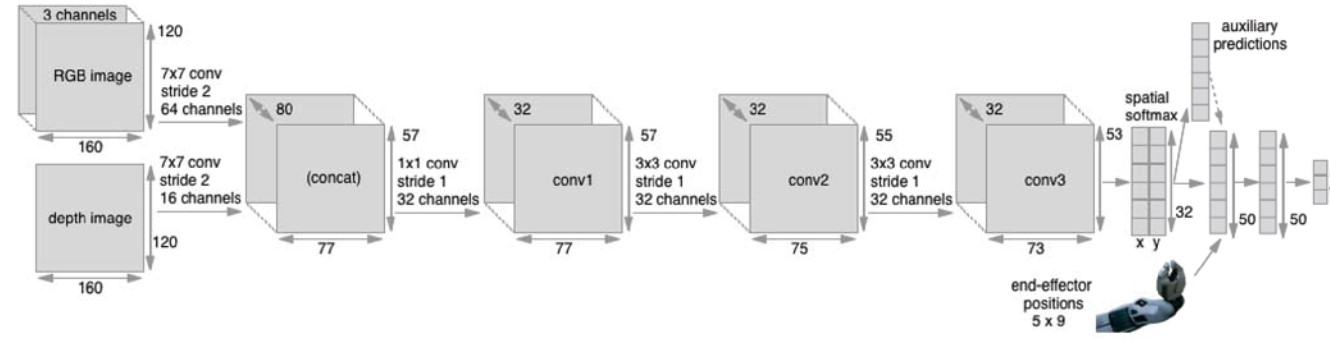
\includegraphics[width=0.9\textwidth]{figures/images/deep_imitation_bc/deep_imitation_bc.jpg}
    \caption{Architecture proposed in~\cite{zhang2018deep_vr_teleoperation}}
    \label{fig:deep_bc}
\end{figure}

% \usepackage{graphicx}
% \usepackage{hhline}


\begin{table}
    \centering
    \caption{Statistics of Training set, and Test Success rate~\cite{zhang2018deep_vr_teleoperation}}
    \label{table:deep_vr_teleoperation_results}
    \resizebox{\linewidth}{!}{%
    \begin{tabular}{|c|c|c|c|c|c|c|c|c|c|c|} 
    \hline
    \textbf{Task} & \textbf{Reaching} & \textbf{Grasping} & \textbf{Pushing} & \textbf{Plane} & \textbf{Cube} & \textbf{Nail} & \begin{tabular}[c]{@{}c@{}}\textbf{Grasp-}\\\textbf{and-}\\\textbf{Place}\end{tabular} & \begin{tabular}[c]{@{}c@{}}\textbf{Grasp-}\\\textbf{Drop-}\\\textbf{Push}\end{tabular} & \begin{tabular}[c]{@{}c@{}}\textbf{Grasp-}\\\textbf{Place-x2}\end{tabular} & \textbf{Cloth} \\ 
    \hhline{|===========|}
    \#demo & 200 & 180 & 175 & 319 & 206 & 215 & 109 & 100 & 60 & 100 \\ 
    \hline
    \begin{tabular}[c]{@{}c@{}}demo duration \\(min)\end{tabular} & 13.7 & 11.1 & 16.9 & 25.0 & 12.7 & 13.6 & 12.3 & 14.5 & 11.6 & 10.1 \\ 
    \hline
    \begin{tabular}[c]{@{}c@{}}Test success rate\\(\%)\end{tabular} & 91.6 & 97.2 & 98.9 & 87.5 & 85.7 & 87.5 & 96.0 & 83.3 & 80.0 & 97.4 \\
    \hline
    \end{tabular}
    }
    \end{table}